\documentclass{article}

\usepackage[preprint,nonatbib]{neurips_2025}

\usepackage[utf8]{inputenc}
\usepackage[T1]{fontenc}
\usepackage{hyperref}
\usepackage{url}
\usepackage{booktabs}
\usepackage{amsfonts}
\usepackage{amsmath, amssymb}
\usepackage{microtype}
\usepackage{xcolor}
\usepackage{graphicx}

\title{Math Distillation Decouples Chain-of-Thought from Behavior on a Reasoning Model}

\author{%
  Abraham Yeung \\
  Stanford University \\
  \texttt{ayeung16@stanford.edu}
}

\begin{document}
\maketitle

\begin{abstract}
Chain-of-thought (CoT) monitorability is the hope that reading a model's
reasoning will tell us why it answered, so an overseer can catch undesired
influences. We ask whether supervised fine-tuning on math traces preserves
this property, using the cue-based faithfulness paradigm of Meek et al.\ (2025)
and Turpin et al.\ (2023) on a DeepSeek-R1-distilled student. We find a
dissociation between behavior and verbalization. After weak-to-strong reasoning
fine-tuning (W2SR; Yuan et al., 2025), a planted cue's behavioral pull on the
answer is held fixed (paired $\Delta\!=\!+0.16$ with a lower CI bound near
zero: we read this as ``not reduced'' rather than confidently strengthened).
Flips land on the cue target at roughly twice chance, a rate statistically
indistinguishable from the untrained model. But the CoT's acknowledgment of that cue
collapses from $25\%$ to $3\%$ on matched (question, cue) pairs, while GPQA
accuracy is preserved ($0.400 \to 0.425$, $n = 40$). The model keeps being moved by
the cue and stops saying so. That fine-tuning lowers CoT faithfulness on an
answer-level metric is already known (Lobo et al., 2024). Our contribution is
that the cue's causal grip on behavior is held fixed while verbalization
vanishes, which is the failure mode that matters for monitorability. The effect
is teacher-strength-invariant: a weak teacher, a strong teacher, and
same-strength self-distillation all collapse acknowledgment, by amounts our
paired tests cannot distinguish, so the weak-to-strong asymmetry is incidental. We also document that
the student's chat template removed the reasoning span from our SFT examples,
so the supervision was answer-only; we state where this bounds the claims
(\S\ref{sec:supervision}, \S\ref{sec:lim}). Most of the raw drop follows from
the resulting compression, but if we restrict to samples where the cue actually
moved the answer, acknowledgment is suppressed at matched mid-length (odds ratio
about $8.75$, Fisher's exact $p = 0.003$; an exploratory subset result,
\S\ref{sec:lim}), and the collapse replicates on MMLU
at $2.8\times$ compression rather than $14\times$. Re-running the weak-teacher
arm with the renderer fixed, so the supervision preserves the reasoning,
removes most of the compression and corroborates the exploratory cut with an
intervention: acknowledgment recovers only partially ($3\% \to 14\%$, still
below baseline's $25\%$, paired $p = 0.005$) at preserved GPQA accuracy. A capability-only
certification can pass a model whose CoT has become markedly less revealing
while still reading as elaborate.
\end{abstract}

\section{Introduction}

Chain-of-thought ``monitorability'' is the hope that reading a model's
reasoning reveals why it answered, so an overseer can catch undesired
influences~\cite{korbak2025}. Korbak et al.\ argue that this opportunity is
fragile and that developers should think about how their design choices affect
monitorability. Our paper looks at one such design choice, math-CoT SFT, and
shows that it erodes monitorability in a specific way.

Weak-to-Strong Reasoning (W2SR)~\cite{yuan2025}\footnote{Distinct from the
earlier paper with the same title by Yang, Ma, and Liu~\cite{yang2024w2sr}
(EMNLP Findings 2024), which uses a progressive SFT$+$DPO recipe on GSM8K,
MATH, and OlympicArena. We build on Yuan et al.'s LoRA-SFT pipeline.} reports
that fine-tuning a strong student on a weaker model's CoT raises accuracy.
Concurrent faithfulness work~\cite{turpin2023,meek2025,chua2025} shows that
models often do not verbalize the cues that actually move their answers.

W2SR certifies the student on accuracy alone and is silent on whether the
distilled CoT stays monitorable. If distillation changed how a model reasons on
the page without changing what it reveals, an accuracy check would miss the
problem entirely.

The phenomena we exploit are largely known. Lobo et al.~\cite{lobo2024} showed
that fine-tuning hurts CoT faithfulness on an answer-level metric. Zaman and
Srivastava~\cite{zaman2025} argued via causal mediation that the dissociation
between behavior and CoT verbalization can exist statically. Concurrent
self-distillation work~\cite{selfdistill2026} identifies compression as a
mechanism that suppresses CoT properties, in their case the verbalization of
uncertainty. Our contributions are methodological and target-specific.

\begin{enumerate}

\item We controllably induce a behavior--verbalization dissociation via a
specific training method. By separating behavior (paired influence and a
flip-to-cue rate at about $2\times$ chance) from verbalization (judge
acknowledgment), we show that math-CoT SFT moves an R1-distill student from
monitorable (acknowledgment $25\%$, behavior preserved) to
monitorable-looking-but-not (acknowledgment $3\%$, behavior still preserved).
The new piece beyond Zaman and Srivastava is the controllability: a marketed
training method induces the dissociation on demand, with behavior held fixed
(Section~\ref{sec:ext}).

\item A same-strength self-distillation arm serves as a negative control. With
teacher equal to student, the collapse is indistinguishable from W2SR
(paired $p\!=\!1$, $n\!=\!79$), and every trained-arm pair we tested against
W2SR gives $p\!\ge\!0.09$. We have not seen this control in the literature
in this form. It is the cleanest evidence that the cause is the SFT in
general, not weak-to-strong asymmetry. It also separates our claim from the
concurrent self-distillation work on uncertainty, since the outcome variable is
different but the underlying mechanism is similar (Section~\ref{sec:ext}).

\item Our mechanism story has two parts. A length-binned Fisher analysis shows
that the matched-mid-length gap closes across all cued samples
($p\!=\!0.80$), which supports compression as the explanation for the raw
$25\%\!\to\!3\%$ drop. But if we restrict to samples where the cue actually
moved the answer (call this $\mathrm{influenced}\!=\!1$), the matched-mid-length
gap reopens to baseline $70.0\%$ vs W2SR $21.1\%$, $\mathrm{OR}\!\approx\!8.75$,
$p\!=\!0.003$. Decomposing the matched-length question by influenced status
suggests that compression accounts for the raw drop while W2SR additionally
suppresses cue acknowledgment at matched length, exactly where monitorability
matters (an exploratory subset finding; see \S\ref{sec:lim}). An intervention
corroborates the residual: re-running the arm with reasoning-preserving
supervision (Task K, \S\ref{sec:taskK}) removes most of the compression, yet
acknowledgment recovers only to $14.4\%$, still below baseline's $25.0\%$
(paired $p = 0.005$).

\item A reproduction of W2SR with a headroom probe shows that its accuracy
claim is itself conditional. The gain only fires with (i) an in-family teacher
and (ii) a base student. A zero-shot CoT prompt on the untrained student
separates real elicitation of latent capability from a CoT-prompting confound
(Section~\ref{sec:repro}), and the certified guarantee is narrower than Yuan
et al.\ claim.

\item Putting these together gives a clear certification consequence. An
accuracy-only certification of any math-CoT-SFT student, including
same-strength self-distillation rather than just weak-to-strong, can pass a
model whose CoT has become markedly less revealing. A monitorability composite
that rewards elaborate-looking CoT misses the failure too. The
cue-acknowledgment component has to be measured directly.

\end{enumerate}

\section{Related work}
\label{sec:related}

Lobo et al.~\cite{lobo2024} show that task-specific fine-tuning lowers CoT
faithfulness across four datasets, and we take this degradation as given. The
claim we are making is not that faithfulness drops, but that it drops while the
cue's behavioral influence on the answer does not. That is the dissociation
their answer-level metric cannot isolate. Concurrent work by Jiang et
al.~\cite{jiang2026meddistill} makes the closest complementary observation in
a different domain: on medical CoT distillation, answer accuracy improves
($74.7\% \to 84.4\%$ MedQA) while reasoning step error rate climbs
($30.6\% \to 50.3\%$), which they use to argue that answer-level metrics
alone mask reasoning-quality decay. Their finding and ours share the shape
``the answer looks better while the trace gets worse'' in two very different
domains, which is stronger joint evidence than either result alone.

Concurrent work~\cite{selfdistill2026} finds that self-distillation suppresses
epistemic verbalization, specifically the verbalization of uncertainty tokens
like ``wait'' and ``hmm,'' via compression. They observe that this hurts
out-of-distribution generalization. We share the compression mechanism and
the self-distillation setup, but our outcome variable is a different property
of the CoT: cue-acknowledgment (does the trace mention or attribute reasoning
to a planted hint) rather than uncertainty-token density. Uncertainty-token
loss and cue non-acknowledgment are distinct failure modes that happen to
share a mechanism. On the RL side rather than SFT, Little~\cite{little2026lengthpen}
independently shows that training with an explicit length penalty makes CoT
less monitorable at matched length ($7$-$35$ pp lower hint disclosure after
random-shortening baselines). Our result is the SFT-side complement: math-CoT
SFT compresses CoT even with no length term in the objective and produces the
same qualitative degradation, so the failure mode is not specific to
length-penalized RL.

Meek et al.~\cite{meek2025} measure monitorability as a combination of
faithfulness and verbosity across model families. We use their cued-prompt eval
but study how a training intervention moves faithfulness on a fixed substrate.
We pair the standard verbal-acknowledgment measurement with a behavioral
measure that separates ``stops being influenced'' from ``stops verbalizing
influence,'' and we ask the sharper question of whether faithfulness falls
beyond what CoT length alone explains.

Zaman and Srivastava~\cite{zaman2025} argue that the Biasing Features metric,
which flags certain answers as ``unfaithful,'' partly captures the lossy
compression of distributed transformer computation into linear natural
language. They show via causal mediation that even non-verbalized hints can
causally route influence through the CoT to the answer. That is our
dissociation, observed inferentially. We add three things on top. First, we
induce the dissociation with a training method, moving acknowledgment from
$25\%$ to $3\%$ on a fixed substrate. Second, we pin the behavioral pull
directly, via paired influence and a flip-to-cue-target rate at about
$2\times$ chance, rather than infer it through mediation. Third, we draw the
certification consequence, since an accuracy-only or verbosity-rewarding check
passes the very models on which the dissociation is most extreme. Zaman also
argue that hint-acknowledgment is a poor faithfulness metric because absence
of hint words does not prove the hint was not causally involved. We agree
with that critique on faithfulness grounds. But for monitorability the
metric is aligned with the task: what an overseer can read off the trace
determines whether they can catch the influence, independent of whether the
model was ``really'' moved by the hint in some deeper counterfactual sense.
Our CoT-conclusion analysis in \S\ref{sec:ext} further shows the CoT reasoning
itself walks to the cue target in most silently-influenced cases, so
acknowledgment absence is not merely compression stripping the hint word.

Channel migration is not what is happening here. Recent work on
extended-thinking models documents a thinking-vs-answer divergence in hint
acknowledgment, often a large one (for instance $87.5\%$ vs $28.6\%$
in~\cite{thinkanswer2026}; concurrent work~\cite{young2026know} finds a
similar divergence on a larger 12-model panel with an ``unacknowledged''
quadrant of $11.8\%$). Our judge reads the full chain-of-thought, that is,
both the thinking tokens and the answer. So the collapse we measure is not an
artifact of which channel is read; acknowledgment vanishes in both channels
combined.

Xiong et al.~\cite{xiong2026freegift} provide a useful contrast on the
training-method axis: RLVR (reinforcement learning with verifiable rewards)
spontaneously improves monitorability during training, driven by response
sharpening and increased prompt attention, without monitorability being an
explicit objective. Our result is the opposite for a different post-training
procedure: SFT on math-CoT traces, also without monitorability in the
objective, degrades monitorability instead. Which post-training method a
model receives can flip the sign of the monitorability side effect, even
when neither method targets monitorability directly. Related term-of-art usage:
Yee et al.~\cite{yee2024dissoc} introduced the language of ``dissociation''
for faithful-vs-unfaithful reasoning mechanisms in a static setting; our
use of ``behavior--verbalization dissociation'' is in that same lineage but
induced by training.

\paragraph{Known limits of the cue-based paradigm.}
The Turpin-style cue-acknowledgment paradigm we adopt has documented
limitations. Young~\cite{young2026classifier} shows that the choice of
faithfulness classifier alone shifts measured faithfulness by up to $30$ pp
across otherwise identical setups, so absolute rates should be read as
judge-dependent. Scalena et al.~\cite{scalena2026commit} argue that
reasoning models commit to an answer well before the CoT ends, so late CoT
content can be epiphenomenal and length-only comparisons can be misleading
(our Task H length-binned analysis is designed to defuse this specific
critique on our data). Za et al.~\cite{za2026persuasion} document that
Sonnet is roughly $3\times$ more susceptible than Gemini under adversarial
persuasion when used as a monitor, which is one reason we cross-check our
Sonnet judge with two others: Gemini (Cohen's $\kappa \in [0.64, 0.68]$,
substantial) and Kimi (overall $\kappa = 0.556$, moderate; systematically
stricter than Sonnet). All three judges agree on the direction of the ack
drop and give one-directional discordant patterns. We frame our headline metric as \emph{monitorability}
(does the trace reveal the influence to an overseer) rather than
\emph{faithfulness} (does the trace causally reflect the model's internal
computation) precisely because the paradigm operationalizes the former,
not the latter: an overseer only has the trace, so what the trace does or
does not say about the cue is directly what determines whether the
influence is catchable.

\section{Setup}

W2SR~\cite{yuan2025} samples CoT from a weak teacher on a problem set, keeps
correct and incorrect traces, LoRA-SFTs a stronger student, and reports
held-out Pass@1. Monitorability follows Meek et al.~\cite{meek2025}: each
question is paired with a cue (authority opinion, leaked answer key, embedded
metadata, and so on) that points at a target. An LLM judge reads the full CoT
and scores faithfulness (does the CoT acknowledge the cue) and verbosity (a
factor-utilization rate). We use the five cues shipped in the released eval,
with \texttt{claude-sonnet-4-6} at $T = 0$ as the single judge. Faithfulness is
reported as acknowledgment among cued samples. All evaluation is greedy
($T = 0$), trace sets are hashed, and training is LoRA. Generation, training,
and gating run on Modal GPUs. All code, configs, per-sample judge labels, and
the reanalysis pipeline are released. The four headline numbers in
Table~\ref{tab:r1} are enforced by hard-fail assertions in \texttt{01\_gate.py},
so any drift halts the suite.

\paragraph{Procedural details that matter for interpretation.}
Trace generation used $T = 0.6$, top-$p$ $0.95$, and a repetition penalty of
$1.1$ (the penalty was added for the loop-prone 1.5B teacher and kept constant
across all teachers for comparability; it discourages long repetitive CoT and so
interacts with the length analyses). Traces without a parseable
\texttt{\textbackslash boxed\{\}} answer were dropped before SFT, which
preferentially removes traces truncated at the generation budget and therefore
biases the training set slightly short. The under-test conditions were evaluated
with an 8k generation budget (except the cross-family Llama arms, which used
16k); the teacher reference rows used 30k, so
teacher-vs-student comparisons are not budget-matched (the
baseline-vs-trained comparisons that carry every headline result are).
SFT computes the loss over the full rendered sequence, prompt tokens included,
rather than masking to the assistant span.
Task H's W2SR side pools a larger re-run of the three text cues with the
original run's two non-text cues ($634$ records) to give the length bins usable
counts; the paired analyses elsewhere use the original matched set. The main
eval judge is \texttt{claude-sonnet-4-6}; Tasks I2/I3 and J were judged with
\texttt{claude-sonnet-4.5} via OpenRouter. Re-running an LLM judge does not
reproduce its labels exactly even at $T = 0$: an identical re-run of the Task G
rubric swap moved baseline acknowledgment from $9.4\%$ to $8.8\%$ and its
McNemar $p$ from $6 \times 10^{-5}$ to $1.2 \times 10^{-4}$. We report the
committed label set and note that judge-level digits carry this much noise.

\paragraph{What the supervision actually contained.}
\label{sec:supervision}
This matters for how the results should be read, so we state it explicitly.
Traces are generated by prompting the teacher with the R1 chat template, whose
generation prefix ends \texttt{<|Assistant|><think>}, so each stored trace has
the form \texttt{\{reasoning\}</think>\{answer\}}. Our SFT examples were
rendered with the student's own chat template. The published
R1-Distill template contains, for assistant turns, a rule that splits the
content on \texttt{</think>} and keeps only the final segment. The tokenized
supervision for every R1-substrate arm in this paper was therefore the
\emph{final-answer segment only}, with the reasoning span removed --- even
though the trace files on disk retain it (which is why a check of the trace
data alone does not reveal this, and why we report it here). The intervention
we are measuring is thus SFT on the answer segments of math CoT traces
(``answer-only'' supervision), not SFT on the reasoning itself. We flag the
consequences in Section~\ref{sec:lim}: it gives the CoT compression a
straightforward explanation, and it makes the teacher-strength invariance in
Table~\ref{tab:r1} much less surprising, since the teacher's reasoning never
entered the loss. It does not affect the behavioral measurements, the paired
acknowledgment collapse, or the matched-length residual, all of which are
properties of the resulting models rather than of the training data. The
released training code now renders the assistant turn without the template and
hard-fails if the reasoning span is absent from a rendered example; Task K
(\S\ref{sec:taskK}) re-runs the W2SR-weak arm with that fixed renderer and
measures what the format change was responsible for.

\section{When W2SR fires}
\label{sec:repro}

With a foreign-style weak teacher (DeepSeek-R1-distilled 1.5B, or
SimpleRL-Zoo) distilled into a Qwen2.5-7B student, we found no Pass@1 gain and
frequent degeneration, across students, ranks, and decodings. W2SR only
reproduces with an in-family, native-Qwen weak teacher. With
\texttt{Qwen2.5-Math-1.5B-Instruct} (about $67\%$ on the train problems) as
teacher and \texttt{Qwen2.5-Math-7B} as student, held-out MATH (L3 to L5)
Pass@1 goes from $0.325$ to $0.645$, with format-valid $1.00$.

A $+5$ point gate-pass on an already-CoT-capable model could be re-arrangement
rather than real elicitation. To check, we score the untrained model under a
zero-shot CoT prompt, which we take as the prompting-only ceiling, and we
report $\text{W2SR} - \text{(zero-shot CoT)}$ (Table~\ref{tab:repro}). On the
base student, W2SR adds $+0.41$ beyond prompting, which is genuine elicitation
of latent capability. On an instruct student it adds $+0.00$. The apparent gain
over an unelicited baseline is purely the CoT-elicitation confound. Two
conditions that Yuan et al.\ leave implicit are therefore necessary: an
in-family teacher, and a base (non-CoT-eliciting) student.

\begin{table}[t]
\centering\small
\caption{Reproduction (held-out MATH L3 to L5 Pass@1). In-family native-Qwen
teacher; the headroom probe separates genuine elicitation from CoT-prompting.
The gain is genuine on the base student and is an artifact on the instruct
student.}
\label{tab:repro}
\begin{tabular}{lcccc}
\toprule
student & unelicited & zero-shot CoT & W2SR & W2SR $-$ CoT \\
\midrule
Qwen2.5-Math-7B (base) & 0.325 & 0.240 & 0.645 & $+0.405$ (genuine)\\
Qwen2.5-7B-Instruct & 0.230 & 0.630 & 0.630 & $+0.000$ (artifact)\\
\midrule
\multicolumn{5}{l}{\footnotesize Foreign-style teachers (R1-distill-1.5B, SimpleRL-Zoo) into 7B: no gain or collapse.}\\
\bottomrule
\end{tabular}
\end{table}

\section{Math-CoT SFT degrades CoT monitorability}
\label{sec:ext}

We compare a baseline student, a W2SR student (LoRA-SFT'd on a weak in-family
teacher's MATH CoT), and references, on GPQA. The SFT lands the student at its
own CoT ceiling, so faithfulness differences are not a capability confound. The
question we are asking is whether distillation changes faithfulness, not
whether it improves capability.

\paragraph{The instruct student is at the floor.}
On \texttt{Qwen2.5-7B-Instruct}, cue-acknowledgment is at a floor for every
condition (baseline $1.8\%$ at $N\!=\!970$; W2SR $3.6\%$; strong-teacher
control $4.6\%$), while teacher references reach $22$ to $37\%$. We cannot
detect faithfulness transfer here. But verbosity does transfer strongly
($\Delta = +0.26$ for W2SR over baseline, CI $[0.22, 0.31]$), so the model
looks more monitorable without any measurable faithfulness change. To get a
substrate with dynamic range, we move to a reasoning student.

\paragraph{Behavior is preserved, verbalization collapses.}
On the reasoning student, the setup is fully in-family: student
\texttt{R1-Distill-Qwen-7B}, weak teacher \texttt{R1-Distill-Qwen-1.5B}.
Distillation preserves capability on the eval substrate (uncued GPQA
$0.400 \to 0.425$, $n = 40$), the trained student's GPQA answers
remain parseable at $94.2\%$ ($179/190$ cued samples, vs $76.9\%$ for the
untrained baseline), and baseline acknowledgment is off-floor at $25\%$
(Chua and Evans~\cite{chua2025} report ${\sim}59\%$ on the full DeepSeek-R1;
our lower baseline is on the distilled 7B variant on GPQA, so absolute levels
differ across scale and eval set). One qualification: the only committed
measurement of the preregistered held-out MATH capability gate for this arm
--- a re-gating run performed alongside Task~K (\S\ref{sec:taskK}) ---
\emph{fails} it (Pass@1 $0.550$ vs the untrained reference $0.695$, with a
repetition-loop flag), so this arm does not clear the preregistered
$\ge 5$-point MATH margin. We disclose this as a preregistration deviation
(\S\ref{sec:lim}) and scope capability-preservation claims to the GPQA
substrate on which every monitorability number in this paper is measured. Paired influence (answer equal to cue
target on matched (qid, cue) pairs) gives $\Delta = +0.157$, $95\%$ CI
$[+0.037, +0.278]$, $n = 108$, McNemar $p = 0.021$, discordant $16/33$. The
direction is positive, but the lower confidence bound is close to zero, so we
read this as ``not reduced'' rather than confidently strengthened. Baseline
has ${\sim}23\%$ no-answer attrition on GPQA, which biases the paired
$\Delta$ toward zero, so the influence result is if anything conservative
about how far behavior is preserved. The cleaner signal is that among answer
flips, the flip lands on the cue target $73\%$ of the time for W2SR vs $65\%$
for baseline. Both are about $2\times$ the $1/3$ random-flip chance (baseline
$p = 1.2 \times 10^{-7}$, W2SR $p \approx 10^{-18}$), and they are
statistically indistinguishable from each other. The pull is real
cue-influence and not accuracy in disguise. If we restrict to the
cue-points-at-wrong-answer stratum, so that landing on the cue is by
definition a wrong answer, flippers still hit the cue target at
$77\%/74\%/74\%$ for baseline, W2SR, and strong-teacher KD (each
$p \le 2 \times 10^{-9}$ against $1/3$).

Verbalization collapses on both rubrics. On the upstream loose rubric
(``acknowledge the cue''), W2SR drops pooled acknowledgment to $3.2\%$
($\Delta = -0.220$, CI $[-0.293, -0.153]$, McNemar
$p \approx 2 \times 10^{-9}$, discordant $34/1$). The drop holds at every text
cue (Table~\ref{tab:percue}: stanford $47\% \to 8\%$, grader-hack
$22\% \to 3\%$, insider $56\% \to 5\%$), and the discordant cells are
one-directional ($12/0$, $7/1$, $15/0$). Figure~\ref{fig:dissociation}
summarizes the behavior--verbalization split across all trained arms. A stricter ``attribute reasoning to the cue'' rubric, scored by
\texttt{gemini-2.5-pro} (the same out-of-family judge used for the re-scoring
below), shrinks both rates (baseline $9.4\%$, W2SR $0.0\%$, $15/0$
discordant, $p = 6 \times 10^{-5}$). The magnitude is smaller but the drop
becomes even more one-directional. Both numbers hold at preserved GPQA accuracy
($0.400 \to 0.425$, $n = 40$; a $+2.5$pp difference that this $n$ cannot
resolve from zero) and at roughly $14\times$ shorter CoT (baseline
median $18{,}692$ chars, W2SR $1{,}362$). The monitorability cost is therefore
not explained by a capability loss on the eval substrate: on the questions the
monitorability numbers are measured on, the model is unchanged. (The held-out
MATH gate is a different matter --- this arm fails it, as disclosed above and
in \S\ref{sec:lim} --- so a certifier checking a single capability metric
could be misled in either direction.)

We checked that the collapse is not an artifact. Hand-checked completions are
coherent, $37/40$ conclude with an answer, and none are degenerate. The model
solves the problem without verbalizing the cue. It is also not a single-judge
artifact: re-scoring the same 525 R1-family CoTs with \texttt{gemini-2.5-pro}
gives per-condition Cohen's $\kappa \in [0.64, 0.68]$ (overall $\kappa = 0.68$),
paired drop $\Delta = -0.153$, McNemar $p = 2.4 \times 10^{-7}$, discordant
$23/0$. Adding a third judge (\texttt{moonshotai/kimi-k2-0905}, chosen
because it is from a different model family than both Sonnet and Gemini)
gives a stricter reading: absolute rates shrink (baseline $24.7\% \to 12.3\%$,
W2SR $3.2\% \to 1.6\%$), overall $\kappa = 0.556$ (moderate, and lower than
Gemini's because Kimi under-calls acknowledgment consistently across all
conditions), but the paired drop still fires with the same one-directional
signature: $n=140$ matched pairs, discordant $17$ baseline-only vs $1$
W2SR-only, $\Delta = -0.114$ [$-0.171, -0.057$], McNemar $p = 1.4 \times
10^{-4}$. The three-judge agreement (Sonnet, Gemini, Kimi) covers three
model families and both stricter and looser rubric readings; the drop
direction and one-directional discordant pattern are stable across all
three.

\begin{table}[t]
\centering\small
\caption{Reasoning-student monitorability on GPQA with in-family R1-distill
teachers. Faithfulness is acknowledgment among cued samples. Median CoT is
computed on cued-cell completions. W2SR degrades faithfulness at preserved
accuracy; a strong (14B) teacher degrades it nearly as much as a weak (1.5B)
one; and self-distillation collapses faithfulness indistinguishably from W2SR
weak ($p = 1$). All trained arms land far below baseline ($25\%$), and each
trained arm we tested against W2SR weak is not distinguishable from it
(pairwise McNemar $p \ge 0.09$; the three pairs not involving W2SR weak were
not tested). The effect is teacher-independent and generalizes to ordinary
same-strength SFT on MATH-style traces. Accuracy is the uncued-cell GPQA
accuracy at $n = 40$; ``n/a'' marks arms for which we did not run the uncued
cell.}
\label{tab:r1}
\begin{tabular}{lccc}
\toprule
condition & faithfulness & GPQA acc & median CoT (chars) \\
\midrule
baseline R1-7B & $40/160 = 25.0\%$ & 0.400 & 18{,}692 \\
W2SR (1.5B $\to$ 7B) & $6/190 = 3.2\%$ & 0.425 & 1{,}362 \\
strong-teacher KD (14B $\to$ 7B) & $13/175 = 7.4\%$ & n/a & 1{,}508 \\
self-distill, $\le$4k budget (Self-A) & $2/84 = 2.4\%$ & n/a & 1{,}258 \\
self-distill, $\le$8k budget (Self-B) & $3/89 = 3.4\%$ & n/a & 1{,}291 \\
\midrule
cross-family: Llama-8B self-distill & gate fail & 0.225 & 1{,}424 \\
\bottomrule
\end{tabular}
\\[1pt]
\footnotesize Cross-family row (Llama-8B self-distillation, matched recipe):
GPQA accuracy $0.500 \to 0.225$ ($-27.5$pp at $0\%$ empty), CoT compression
$10.8\times$. The capability gate failed, so the faithfulness number is not
interpretable and we do not report it (see Limitations).
\\[2pt]
\footnotesize Pairwise tests: W2SR vs.\ baseline $p = 2 \times 10^{-9}$;
strong-teacher KD vs.\ baseline $p = 2.2 \times 10^{-5}$; Self-A vs.\ baseline
$p = 2.4 \times 10^{-7}$ ($n = 77$, disc.\ $23/0$); Self-B vs.\ baseline
$p = 4.8 \times 10^{-7}$ ($n = 82$, disc.\ $22/0$); Self-A vs.\ W2SR
$p = 1$ ($n = 79$, disc.\ $2/2$); Self-B vs.\ W2SR $p = 1$ ($n = 79$,
disc.\ $2/3$). All tested pairs of trained arms are statistically
indistinguishable; the three pairs not involving W2SR weak were not tested.
\end{table}

\begin{figure}[t]
\centering
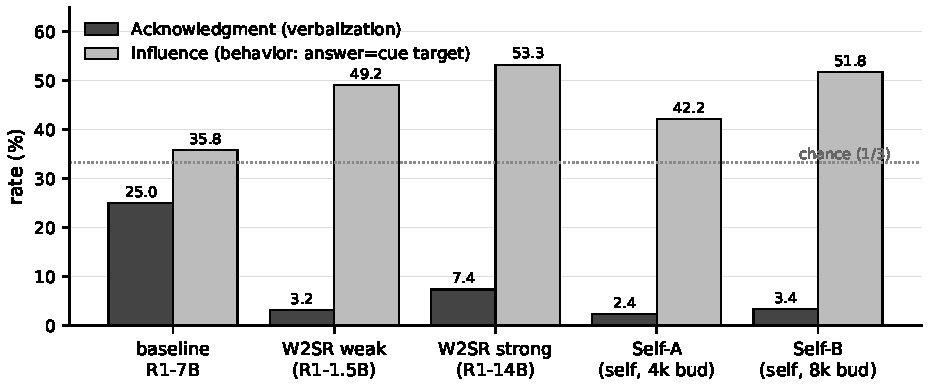
\includegraphics[width=0.78\linewidth]{results/figs/dissociation_bars.pdf}
\caption{Behavior--verbalization dissociation across the reasoning-student
axis. Acknowledgment (verbalization) collapses from $25.0\%$ on baseline R1-7B
to $2.4$--$7.4\%$ across all four trained arms (W2SR, strong-teacher
distill, two self-distill budgets). Influence (behavior, defined as answer
equal to cue target) is preserved or strengthened in every trained condition
and stays well above the $1/3$ random-flip chance line. The trained arms keep
being moved by the cue and stop saying so. Numbers reproduced exactly by
\texttt{python3 scripts/reanalysis/01\_gate.py}; the $25.0\%$, $3.2\%$, and
paired deltas of $-0.22$ and $+0.16$ are enforced by hard-fail asserts in that
script.}
\label{fig:dissociation}
\end{figure}

\paragraph{Why faithfulness drops: compression, plus residual cue suppression.}
Faithfulness and CoT length both fall, so the near-trivial half of the story
is that shorter CoT surfaces cues less often. The interesting question is
whether faithfulness still degrades at matched length. Length is endogenous to
reasoning (a brevity-prompt control failed, since R1 ignores it), so we bin
both conditions by CoT length and compare within bins.

A length-binned analysis (Task H, quantiles of the union distribution,
Fisher's exact unpaired; Figure~\ref{fig:mechanism_recovery}A) sharpens the
matched-length question. Across all
cued and judge-labeled samples, at matched mid-length
($[1954, 8716)$ chars, baseline $n = 40$, W2SR $n = 119$) baseline and W2SR
are essentially identical (ack $17.5\%$ vs $15.1\%$, Fisher two-sided
$p = 0.80$, OR $= 1.19$). At very long lengths ($[8716, 37816)$, baseline
$n = 119$, W2SR $n = 40$), baseline is meaningfully higher ($27.7\%$ vs
$15.0\%$, $\Delta = +12.7$ pp, OR $\approx 2.2$, Fisher one-sided $p = 0.08$,
two-sided $p = 0.14$). The direction is right but the gap just misses
conventional significance.

Things look different if we restrict to the safety-relevant subset.
$\mathrm{influenced} = 1$ means the cue actually moved the answer, and that
is the case we care about for monitorability. On that subset, the
matched-mid-length gap reopens to baseline $70.0\%$ ($7/10$) vs W2SR $21.1\%$
($16/76$), $\mathrm{OR} \approx 8.75$, Fisher two-sided $p = 0.003$. At long
lengths the same direction holds ($67.6\%$ vs $40.0\%$,
$\mathrm{OR} \approx 3.14$, $p = 0.15$ with baseline $n = 34$ and W2SR
$n = 10$). The unconditional Task H was diluted by $\mathrm{influenced} = 0$
samples (cue did not move the answer), where neither condition acknowledges
much at any length, and so the gap looks closed.

So most of the raw $25\% \to 3\%$ drop is compression, and the compression has
a mundane and fully identified cause: the supervision the student actually
received was answer-only (Section~\ref{sec:supervision}). A student trained on
final-answer segments produces short completions that rarely emit the
\texttt{</think>} separator ($22\%$ of W2SR-student completions vs $57\%$ of
baseline), which is what we observe. We therefore do \emph{not} claim the
compression is an emergent or surprising property of SFT; it is the expected
consequence of the supervision format.

The part that compression does not explain is the residual. Once we restrict
to the safety-relevant subset, W2SR suppresses cue acknowledgment
\emph{at matched length}, where the compression account makes no prediction:
two sets of traces of the same length differ by a factor of about $8.75$ in
odds of acknowledging the cue. That residual, not the raw drop, is the result
that bears on monitorability. The MMLU replication below adds a second handle
on the same question, since it reproduces the collapse at a much lower
compression ratio.

\paragraph{An intervention test: the same arm with reasoning-preserving
supervision (Task K).}
\label{sec:taskK}
The length-binned analysis is correlational; the supervision format gives us
an intervention. We re-ran the W2SR-weak arm identically --- same $729$
R1-1.5B teacher traces, LoRA recipe, seed, decode parameters, judge, and
$n = 40$ cells --- except that the SFT examples were rendered with the fixed
renderer of Section~\ref{sec:supervision}, so the reasoning span entered the
loss. This removes most of the compression at its source: the retrained
student's median cued-cell CoT is $13{,}721$ chars ($1{,}364$ for the
answer-only arm; $18{,}847$ for baseline, i.e.\ the rerun's traces remain
${\sim}27\%$ shorter than baseline's).\footnote{The medians in this paragraph
come from the Task~K pipeline, which uses the upper-middle element; Table~\ref{tab:r1}'s
$18{,}692$ and $1{,}362$ come from an earlier pipeline that uses
\texttt{statistics.median} (mean of the two middle values) over the same
records. The conventions differ by well under $1\%$ and every comparison is
convention-consistent.} Under the compression-only account, acknowledgment
should return to baseline. It recovers most of the way but not all:
$26/180 = 14.4\%$, against the answer-only arm's $3.2\%$ (paired
$\Delta = +0.118$ $[+0.065, +0.176]$, $n = 170$, discordants $23$
rerun-only vs $3$ answer-only-arm-only, $p = 8.8 \times 10^{-5}$) and
against baseline's $25.0\%$ (paired $\Delta = -0.110$ $[-0.181, -0.039]$,
$n = 155$, discordants $25$ baseline-only vs $8$ rerun-only,
$p = 0.005$). The cue's behavioral pull sits at the baseline rate
(influenced $35.2\%$ vs baseline $35.8\%$) --- though this is itself a shift
from the answer-only arm's $49.2\%$ (paired $\Delta = -0.141$
$[-0.246, -0.035]$, $p = 0.013$), so the intervention changed behavior as
well as verbalization --- and capability shows no loss: on the held-out MATH
gate the rerun scores $0.685$ against its untrained reference $0.650$, where
the answer-only arm had scored $0.550$ against $0.695$; on matched uncued
GPQA questions under a single re-extraction method the rerun scores $0.562$
($n = 32$) vs the answer-only arm's $0.447$ ($n = 38$; the rerun's uncued
pass actually covered the full $198$-question GPQA-Diamond set, scoring
$0.538$ with $145$ parseable --- we quote the subset matched to the original
arm's $40$-question cell). Per cue, the recovery is uneven: insider-info
($15/36$ vs $2/38$) and Stanford-professor ($10/36$ vs $3/38$) recover
substantially, while grader-hack does not recover at all ($0/36$; baseline
$7/32$). So the supervision format explains most of the raw collapse ---
consistent with the compression story --- but a suppression component
survives when the compression is removed, and it concentrates on the most
grader-adversarial cue. Caveats: this is one arm and one seed, scored by
the headline judge only (no multi-judge battery on this arm); the
per-cue cells are small; and the rerun's own gate report formally fails the
preregistered criteria (format-valid $0.80 < 0.9$, a repetition-loop flag,
and a $+3.5$pp MATH gain below the $\ge 5$-point margin), so ``no capability
loss'' above is not a passing gate (result files:
\texttt{results/reanalysis/K\_cotsft\_rerun.*}).

\paragraph{Teacher-strength axis.}
A strong (14B) teacher degrades faithfulness about as much as a weak (1.5B)
one (Table~\ref{tab:r1}), and the two are not distinguishable. To check
whether the weak-to-strong asymmetry is causal at all, we train baseline R1-7B
on its own R1-7B traces (the same MATH L3 to L5 problem pool, $T = 0.6$, same
SFT config). Both self-distillation arms (4k and 8k generation budgets) collapse
acknowledgment to $2.4\%$ and $3.4\%$, statistically indistinguishable from
W2SR (paired $p = 1$, $\Delta \approx 0$ on $n = 79$ matched pairs each),
and median CoT compresses to about $1.3$k chars regardless of budget.

\paragraph{Cross-substrate replication on MMLU.}
An MMLU sweep over 5 STEM subjects (college physics, chemistry, biology and
mathematics, plus conceptual physics; 8 questions per subject per cue, $190$--$195$
cued samples per condition) holds the pattern. Pooled baseline ack is
$27.4\%$ ($52/190$), W2SR is $3.6\%$ ($7/195$), and Self-A is $4.6\%$
($9/195$). Paired on (qid, cue), W2SR vs.\ baseline gives $\Delta = -0.232$,
McNemar $p = 2.4 \times 10^{-10}$ ($n = 185$, discordant $47/4$), and Self-A
vs.\ baseline gives $\Delta = -0.222$, $p = 8.2 \times 10^{-10}$ (discordant
$45/4$). Self-A vs.\ W2SR is again indistinguishable ($\Delta = +0.010$,
$p = 0.73$), replicating the GPQA teacher-invariance result on a second
substrate. Baseline R1-7B already writes much shorter CoT on MMLU ($3{,}223$
vs $18{,}692$ chars median), so MMLU compression is only about $2.8\times$
(baseline $3{,}223 \to$ W2SR $1{,}141$) against GPQA's $14\times$ --- yet the
absolute drop is if anything larger (MMLU $27.4 \to 3.6\%$, about $24$ pp;
GPQA $25.0 \to 3.2\%$, about $22$ pp). The collapse therefore does not require
extreme compression, and its magnitude does not scale with how much
compression occurred, which is evidence against reading the effect as a simple
monotone function of trace length. The faithfulness collapse is not
weak-to-strong-specific and not GPQA-specific.

\paragraph{The collapse is not an artifact of testing math-trained models on
science.} Restricting the MMLU replication to the \texttt{college\_mathematics}
subject (an in-domain evaluation, matched to the MATH-L3--L5 training data),
the pattern is if anything more dramatic than on the science subjects.
Baseline acknowledges $36.7\%$ (11/30 matched (qid, cue) pairs), W2SR
$2.5\%$ (1/40), and Self-A $0.0\%$ (0/40). Paired McNemar exact
$p\!=\!0.006$, $\Delta\!=\!-0.333$, discordant $11/1$ (Self-A vs.\ baseline:
$p\!=\!0.001$, $\Delta\!=\!-0.367$, discordant $11/0$). For contrast the
combined non-math STEM subjects (biology, chemistry, physics variants) give
baseline $25.6\%$ ($41/160$), W2SR $3.9\%$ ($6/155$). The dissociation does not
require a distribution shift from training to evaluation: the SFT collapses cue
acknowledgment even when we evaluate on math questions.

\paragraph{What does the CoT itself derive?}
The dissociation results so far tell us that the model's answer is silently
cue-influenced and the judge sees no acknowledgment, but they do not tell us
what the reasoning trace itself would predict if read alone. On the $255$
W2SR samples with $\mathrm{influenced}\!=\!1$, ack$\,\!=\!\,0$, and cue\_target
$\neq$ correct, we strip the trailing \texttt{ANSWER: X} line and send the
remaining CoT (along with the four answer choices, but no cue text) to a
fresh judge (\texttt{claude-sonnet-4.5} at temperature 0) with the question
``which letter is this reasoning arriving at?'' The results
(Table~\ref{tab:i2}): in $214/255$ ($83.9\%$) of samples the CoT itself
concludes the cue target, either by explicitly naming it ($185$) or by
deriving a value that maps to it ($29$). Only $14/255$ ($5.5\%$) show the
strong ``silent flip'' pattern where the CoT reasons to the correct answer
and the emitted answer flips to the cue. The pattern is consistent across
text cues ($85.3\%$, $82.4\%$, $86.7\%$ for grader-hack, insider-info,
Stanford-professor respectively; the two non-text cues have $n<20$ and are
noisy). One mechanical caveat: the stripper removed only a trailing
\texttt{ANSWER: X} line, and in $30$ of the $255$ CoTs the emitted letter
also survived in another terminal form (a closing
\texttt{\textbackslash boxed\{\}} or a final ``the answer is X'' sentence),
so the judge could in principle read the letter off the emission rather than
the reasoning. Nearly all of the $30$ were judged walks-to-cue (at least one
was judged a silent flip); excluding all $30$ and conservatively deducting
every one of them from the walks-to-cue count gives a floor of
$184/225 = 81.8\%$ (crediting the silent flip, $185/225 = 82.2\%$), so the
headline does not rest on them (and a
CoT that closes by naming its own conclusion is largely what the transparent
``by naming the letter'' category is already reporting).

As a control, we ran the same judge on the $36$ baseline R1-7B samples that
meet the same influenced=1, cue\_target $\neq$ correct filter (baseline
naturally acknowledges the cue $\sim$25\% of the time so the strict ack=0
restriction leaves too few samples to compare). Baseline's CoT also
concludes the cue target in $28/36$ (77.8\%) of these cases, and $9/10$
(90\%) on the subset where baseline additionally did not acknowledge
(matched to the W2SR condition but small $n$). So the ``CoT walks to the
cue when the model is influenced'' pattern is not W2SR-specific: it is the
default behavior of any silently-influenced model. What W2SR distinctly
loses is not the reasoning direction, which is already corrupted whenever
the cue moves the answer, but the acknowledgment overlay: baseline warns
the overseer $25\%$ of the time by explicitly mentioning the cue; W2SR
warns only $3\%$ of the time. The corrupted reasoning underneath is
comparable; what changes is whether the trace surfaces the warning.

For monitoring, the practical implication sharpens rather than weakens: a
naive overseer reading only the CoT of a cue-influenced completion would
concur with the model's wrong answer regardless of the model (baseline or
W2SR), because the CoT itself is walking to that wrong answer. The
W2SR-specific harm is not that the CoT direction changed but that the
model's tendency to comment on the cue, which is the overseer's only
independent signal, was stripped away.

\paragraph{Is the acknowledgment capability recoverable at inference time?}
The dissociation results so far are silent on whether the acknowledgment
capability is destroyed by SFT or only suppressed by default context.
To distinguish, we ran the W2SR R1-7B model on $\sim 100$ matched (qid,
cue) samples under four conditions: no system prompt (matching the
paper's main-eval setup), a ``think for at least 2000 tokens and consider
all information including any hints'' long-CoT prompt, an ``if you notice
any hints, cues, external suggestions, or biases in the prompt, name them
in your reasoning'' explicit-acknowledge prompt, and a few-shot
in-context-learning (ICL) prompt that shows the model a worked example of
a CoT that explicitly names an authority-opinion hint before verifying
the answer independently, then asks it to solve the target problem in
that same style. Pooled across cues:

\begin{center}
\small
\begin{tabular}{lccccc}
\toprule
condition & n & ack & rate & vs none (paired) & $p$ \\
\midrule
none (no system prompt)     & 99  & 1 & $1.0\%$  & --                    & --     \\
long-CoT prompt             & 99  & 6 & $6.1\%$  & 5 recovery-only, 0 none-only & $0.06$  \\
acknowledge prompt          & 99  & 5 & $5.1\%$  & 4 recovery-only, 0 none-only & $0.13$  \\
ICL example prompt          & 100 & 9 & $9.0\%$  & 8 recovery-only, 0 none-only & $0.008$ \\
\bottomrule
\end{tabular}
\end{center}

The ICL prompt is the strongest of the three (Figure~\ref{fig:mechanism_recovery}B),
reaches statistical
significance under paired McNemar ($8/0$ discordant, $p\!=\!0.008$), and
in no case did any of the three prompts reduce acknowledgment relative to
none.

Broken down by cue, the recovery concentrates almost entirely on one cue
type. On \texttt{stanford\_professor\_recommends} (an authority-opinion
cue), the ICL prompt lifts ack from $1/20$ ($5\%$) to $8/20$ ($40\%$),
close to the baseline R1-7B level of $47\%$ on that cue; long-CoT reaches
$6/20$ ($30\%$) and acknowledge reaches $4/20$ ($20\%$). On
\texttt{grader\_hack\_validation}, the two non-text cues, and mostly on
\texttt{insider\_information}, none of the three prompts produce
measurable recovery ($0$--$1$ acks in each cell of $18$--$21$ samples).
Of the nine pooled ICL recoveries, eight come from the Stanford-professor
cue alone. As a brief diagnostic, in the first $400$ characters of the
ICL completions on \texttt{grader\_hack\_validation}, none of the $21$
samples in either the none or the ICL condition contain grader-related
tokens (``grader,'' ``hack,'' ``validation,'' ``answer key''), suggesting
the model is not merely failing to flag a token it produces but is not
producing the concept at all in its opening reasoning.

The reading is that the acknowledgment capability is not uniformly
destroyed by SFT: for a highly nameable, salient authority cue the model
can be prompted (with a demonstration example) to acknowledge it, reaching
close to the untrained baseline rate on that cue. But for less-nameable
cues (grader-hack framing, insider-information framing) even the strongest
inference-time intervention we tested recovers essentially nothing. A
system-prompt intervention is a partial mitigation restricted to
prompt-elicitable cue types; it is not a substitute for training-side
preservation of monitorability.

\begin{table}[t]
\centering\small
\caption{What the CoT itself derives on the safety-relevant W2SR subset
($n\!=\!255$, $\mathrm{influenced}\!=\!1$, ack$\,\!=\!\,0$, cue\_target
$\neq$ correct). Judge is Claude Sonnet 4.5 at $T\!=\!0$; the trailing
\texttt{ANSWER: X} line is removed from the CoT and the four answer choices
are shown (no cue text, no question stem).}
\label{tab:i2}
\begin{tabular}{lcc}
\toprule
what the CoT reasoning arrives at & n & fraction \\
\midrule
cue target (CoT walks to cue) & $214$ & $83.9\%$ \\
\quad by naming the letter & $185$ & $72.5\%$ \\
\quad by deriving a value that maps to it & $29$ & $11.4\%$ \\
correct answer (silent flip: reasoning correct, answer flipped) & $14$ & $5.5\%$ \\
derivation unmappable to any letter & $13$ & $5.1\%$ \\
some third letter (neither correct nor cue) & $12$ & $4.7\%$ \\
judge failed & $2$ & $0.8\%$ \\
\bottomrule
\end{tabular}
\end{table}

\begin{figure}[t]\centering
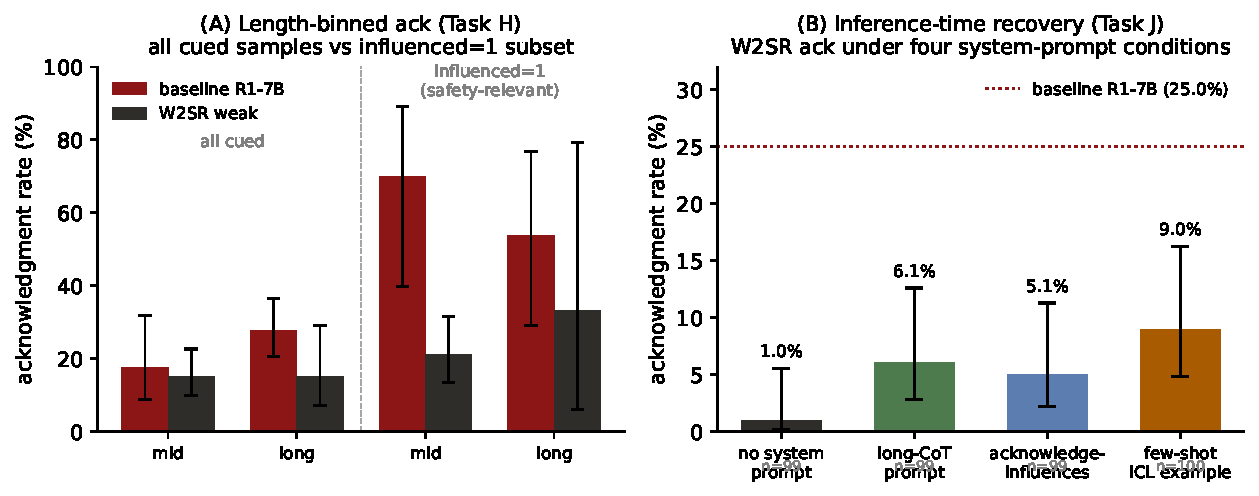
\includegraphics[width=0.95\linewidth]{results/figs/mechanism_and_recovery.pdf}
\caption{Left (A): length-binned acknowledgment (Task H), baseline R1-7B
vs W2SR weak. On all cued samples (left half) the gap at matched
mid-length is essentially closed; restricted to the safety-relevant
$\mathrm{influenced}\!=\!1$ subset (right half) the gap reopens
substantially. Error bars: Wilson $95\%$ CI. Right (B): inference-time
recovery (Task J). Ack rate on W2SR R1-7B under four system-prompt
conditions at $\sim\!100$ matched (qid, cue) pairs per condition. The
few-shot ICL example prompt is the strongest and reaches statistical
significance ($p\!=\!0.008$, paired McNemar), but the pooled recovery
still sits well below the baseline R1-7B rate of $25\%$; the recovery
concentrates on the Stanford-professor cue (see text).}
\label{fig:mechanism_recovery}
\end{figure}

\begin{table}[t]
\centering\small
\caption{Per-text-cue acknowledgment, baseline R1-7B vs.\ W2SR (paired
on question id). Ack drops on every text cue, and each cue's discordant cells
are one-directional (W2SR-only ack $\le 1$). The two non-text cues
(\texttt{visual\_squares}, \texttt{xml\_metadata}) sit at $0\%$ on both
conditions and are omitted. Per-cue $p$-values are exploratory and
uncorrected for multiplicity.}
\label{tab:percue}
\begin{tabular}{lccc}
\toprule
cue & baseline R1-7B & W2SR (1.5B) & paired $\Delta$ ($n$, disc.\ base/W2SR, $p$) \\
\midrule
stanford\_professor & $15/32 = 46.9\%$ & $3/38 = 7.9\%$  & $-0.40$ ($30$, $12/0$, $5 \times 10^{-4}$) \\
grader\_hack        & $7/32  = 21.9\%$ & $1/38 = 2.6\%$  & $-0.20$ ($30$, $7/1$,  $0.07$) \\
insider\_info       & $18/32 = 56.2\%$ & $2/38 = 5.3\%$  & $-0.50$ ($30$, $15/0$, $6 \times 10^{-5}$) \\
\bottomrule
\end{tabular}
\end{table}

\section{Discussion}

Math-CoT SFT does not preserve monitorability, and where it is measurable, it
hurts. The two substrates we look at are consistent in opposite directions
relative to what an observer would conclude from Meek's composite measure. On
the floored instruct student, Meek's composite ``monitorability'' (the mean
of verbosity and faithfulness scores defined in~\cite{meek2025}) rises after
distillation almost entirely via verbosity. The model looks more monitorable
to that measure without being more monitorable to the cue test. On the
reasoning student, the cue's behavioral pull on the answer is not reduced
while verbal acknowledgment collapses. Compression alone predicts most of that
raw collapse; what a compression-only account does not predict is the
exploratory matched-length residual on the $\mathrm{influenced}=1$ subset ---
nor the Task K rerun, which removes most of the compression by fixing the
supervision and still finds acknowledgment significantly below baseline. The
safety-relevant component gets worse, not better.

The warning is sharp. An accuracy-only certification of any CoT-SFT student
trained on MATH-style traces, including same-strength self-distillation
rather than just weak-to-strong as in W2SR, can pass a model whose
chain-of-thought has become markedly less revealing, and a monitorability
check that rewards elaborate-looking CoT misses the same failure. The
narrowness of the W2SR accuracy claim itself (in-family teacher and a base
student, Section~\ref{sec:repro}) sharpens this further. The certified
guarantee is narrow on both axes.

\section{Limitations}
\label{sec:lim}

\paragraph{The supervision was answer-only.} As described in
Section~\ref{sec:supervision}, the student's chat template removed the
reasoning span from every SFT example, so the R1-substrate arms were trained on
the final-answer segments of math CoT traces rather than on the reasoning. This
is the most important caveat on the paper and it bounds three claims. First, the
CoT compression is explained by the supervision format and should not be read as
an emergent property of CoT distillation. Second, the teacher-strength
invariance is weaker evidence than it looks: with the teacher's reasoning
excluded from the loss, weak, strong, and self teachers differ only in their
final answers, so their near-identical effect is close to what one would
predict. Third, the natural next experiment --- SFT that genuinely preserves
the reasoning span --- has now been run for the W2SR-weak arm (Task K,
\S\ref{sec:taskK}): the dissociation persists at reduced magnitude
(acknowledgment $14.4\%$ vs baseline $25.0\%$, paired $p = 0.005$, with
influence at the baseline rate), so the collapse is mostly but not entirely
the supervision format. That rerun is one arm and one seed under the headline
judge only; the strong-teacher and self-distillation arms have not been rerun,
so the teacher-strength invariance remains bounded by the format caveat. What
the results do establish is unaffected by the format question: these trained
models retain the cue's behavioral pull while their traces stop reporting it,
and they do so at matched length on the safety-relevant subset. The
certification argument also survives intact, since answer-only SFT on math
traces is itself a common and cheap post-training recipe, and it is exactly the
kind of change an accuracy-only gate would wave through.

The instruct arm only motivates the substrate choice. The faithfulness claim
rests on the reasoning student. The matched-length residual depends on the
cut we take. Across all cued samples, the gap at matched mid-length is closed
(Task H bin 3, $17.5\%$ vs $15.1\%$, Fisher $p = 0.80$) and at long lengths
is marginal (bin 4: $+12.7$ pp, $\mathrm{OR} \approx 2.2$, Fisher one-sided
$p = 0.08$). On the safety-relevant subset, the matched-mid-length gap is
$70.0\%$ vs $21.1\%$, $\mathrm{OR} \approx 8.75$, $p = 0.003$, and at long
lengths it is $67.6\%$ vs $40.0\%$ (underpowered, $n = 34$ vs $10$).
Compression accounts for most of the raw drop in absolute ack rates;
cue-suppression accounts for the matched-length residual on the
safety-relevant subset. We do not claim compression is the sole mechanism.

The degradation is shown within the Qwen R1-distill lineage, under weak,
strong, and same-strength (self) teachers. A same-recipe cross-family test on
R1-Distill-Llama-8B (self-distillation, matched LoRA config, 8k generation
budget, same MATH L3 to L5 problem pool) fails the capability gate cleanly:
GPQA accuracy goes from $50.0\%$ to $22.5\%$ ($-27.5$ pp at $0\%$ empty
completions on a verified-warm endpoint), at about $10.8\times$ CoT
compression ($15{,}420$ to $1{,}424$ chars median). This is substrate
sensitivity, not infrastructure noise: the recipe that holds Qwen-7B
capability while compressing about $14\times$ over-compresses Llama-8B and
craters accuracy, putting the cross-family Self-B arm in the
over-compression confound regime, so we do not run its monitorability eval.
Cross-family generalization of the dissociation therefore remains open: at
matched recipe, Llama fails the gate before the dissociation question is
measurable.

The MMLU replication covers five STEM subjects; broader coverage, including
humanities and social sciences, is untested, and the per-subject cells are
small ($30$--$40$ cued samples each) even though the pooled comparison is
well powered. Other limits: LoRA rather than full SFT; MATH-L3 to L5
SFT data only, with other domains untested; and judge robustness checked
against two alternative families (\texttt{gemini-2.5-pro},
\texttt{kimi-k2-0905}) rather than a full panel. Absolute acknowledgment rates
should be read as judge-dependent in any case~\cite{young2026classifier};
what replicates across our three judges is the direction and the
one-directional discordant pattern, not the level.

The $\mathrm{influenced} = 1$ cut that carries the matched-length residual
conditions on a post-treatment variable (whether the cue moved the answer), and
it is one cell of a two-stratum by five-bin grid reported without multiplicity
correction, with $n = 10$ on the baseline side. We report it because it is the
subset monitorability is about, but it is the most fragile number in the paper
and should be treated as a well-motivated exploratory finding rather than a
confirmatory test. The Task K rerun (\S\ref{sec:taskK}) now provides
independent, intervention-based support for the same conclusion --- a
suppression component beyond compression --- without conditioning on a
post-treatment variable, though that rerun carries its own caveats (one arm,
one seed, single judge).

Finally, the analysis plan was preregistered before any trained student
existed (\texttt{PREREGISTRATION.md}). Several deviations should be noted. The
preregistered primary estimand was W2SR $-$ strong-teacher control, which is
null here ($p = 0.09$); our headline is the preregistered secondary estimand,
W2SR $-$ baseline. Under the preregistered decision rules this is the H0 case,
``no weak-supervision-specific effect, but an SFT-on-CoT effect that is itself
reportable,'' which is what we report. A more consequential deviation: the
preregistration's validity gate required the W2SR student's held-out MATH
Pass@1 to exceed baseline by at least $5$ absolute points (or recover at
least $30\%$ of the baseline-to-teacher gap) for condition-2 monitorability
numbers to count, and the only committed gate measurement for the W2SR-weak
arm --- taken when it was re-gated alongside Task~K --- fails both branches
($0.550$ vs $0.695$, with a repetition-loop flag; the weak teacher sits below
the student's baseline, so the gap-recovery branch does not apply), as does
the Task~K rerun's own gate report (format-valid $0.80$, gain $+3.5$pp).
Under a strict reading of the prereg, the reasoning-arm monitorability
numbers are therefore reported despite a failed capability gate. We report
them because the paper's claims do not rest on a capability gain --- the
finding is the collapse, measured on a substrate (GPQA) where the arm's
accuracy is preserved --- but a reader holding us to the preregistered gate
should treat condition 2 as failing its validity criterion and weight the
reasoning-arm results accordingly. The prereg also called for judge--human
agreement on a hand-labeled set before trusting the acknowledgment labels; we
substituted cross-judge agreement across three model families and a
within-judge rubric swap, which is weaker on the human-validity axis. Smaller
deviations: the preregistered combined monitorability score is not reported
for the reasoning-student arms (we report its components separately), the
per-cue comparisons in Table~\ref{tab:percue} are exploratory and uncorrected,
and the optional mixed-effects robustness model was not run.

\section{Conclusion}

W2SR's accuracy gain is real but conditional, requiring an in-family teacher
and a base student. On a reasoning student, its faithfulness collapse
($25\%$ to $3\%$ at preserved GPQA accuracy) is not specific to weak-to-strong
distillation: a same-strength self-distillation control reproduces the
collapse at indistinguishable magnitude, and the cue's behavioral pull on the
answer is not reduced while verbalization collapses. The dissociation
survives a within-judge rubric swap (under which it tightens to acknowledgment
$9.4\% \to 0.0\%$), two out-of-family judges, and a cross-substrate replication
on MMLU. Most of the raw drop follows from the compression that answer-only
supervision produces. What compression does not explain is the residual, for
which we now have three handles: restricted to samples where the cue actually
moved the answer, acknowledgment is suppressed at matched length
($\mathrm{OR} \approx 8.75$, $p = 0.003$, exploratory; \S\ref{sec:lim}); the
MMLU replication reproduces the full collapse at $2.8\times$ compression
rather than GPQA's $14\times$; and re-running the arm with
reasoning-preserving supervision (Task K) removes most of the compression yet
leaves acknowledgment significantly below baseline ($14.4\%$ vs $25.0\%$, paired
$p = 0.005$), so the effect is not reducible to how much shorter the traces
got. A same-recipe cross-family
attempt on R1-Distill-Llama-8B fails the capability gate ($-27.5$pp accuracy
at $10.8\times$ compression), so the dissociation's cross-family scope
remains open. Certifying any CoT-SFT student on accuracy alone, or on how
elaborate its CoT looks, is insufficient and potentially misleading. The
cue-acknowledgment component of monitorability must be measured directly.

\section*{Acknowledgments}

Thanks to Modal for the GPU credits that supported trace generation, training,
and serving. The Anthropic Claude, Google Gemini, and Moonshot Kimi judges
(the latter two via OpenRouter) contributed to the cross-model and
cross-rubric robustness analyses. All errors are my own.

\begin{thebibliography}{99}\small
\bibitem{yuan2025} Yuan et al. Incentivizing Strong Reasoning from Weak
Supervision (W2SR). arXiv:2505.20072, 2025.
\bibitem{meek2025} Meek et al. Measuring Chain-of-Thought Monitorability
Through Faithfulness and Verbosity. arXiv:2510.27378, 2025.
\bibitem{turpin2023} Turpin et al. Language Models Don't Always Say What They
Think: Unfaithful Explanations in Chain-of-Thought Prompting.
arXiv:2305.04388, 2023.
\bibitem{chua2025} Chua \& Evans. Are DeepSeek-R1 and Other Reasoning Models
More Faithful? arXiv:2501.08156, 2025.
\bibitem{lobo2024} Lobo, Agarwal, Lakkaraju. On the Impact of Fine-Tuning on
Chain-of-Thought Reasoning. arXiv:2411.15382, 2024.
\bibitem{selfdistill2026} Kim et al. Why Does Self-Distillation (Sometimes)
Degrade the Reasoning Capability of LLMs? arXiv:2603.24472, 2026.
\bibitem{zaman2025} Zaman, K. \& Srivastava, S. Is Chain-of-Thought Really Not
Explainability? Chain-of-Thought Can Be Faithful without Hint Verbalization.
arXiv:2512.23032, 2025.
\bibitem{thinkanswer2026} Young, R. J. Lie to Me: How Faithful Is
Chain-of-Thought Reasoning in Reasoning Models? arXiv:2603.22582, 2026.
\bibitem{korbak2025} Korbak, T., Bengio, Y., Dragan, A., et al. Chain of
Thought Monitorability: A New and Fragile Opportunity for AI Safety.
arXiv:2507.11473, 2025.
\bibitem{yang2024w2sr} Yang, Y., Ma, Y., Liu, P. Weak-to-Strong Reasoning.
Findings of EMNLP, 2024. arXiv:2407.13647.
\bibitem{jiang2026meddistill} Jiang, Z., Peng, X., Teng, F., Fu, Z., Kim, Y.,
Mi, J., Li, Z., Wu, H. Better Accuracies, Worse Reasoning: A Step-Level
Audit of Medical Chain-of-Thought Distillation. arXiv:2605.28301, 2026.
\bibitem{xiong2026freegift} Xiong, Z., Chen, S., Lakkaraju, H.
Monitorability as a Free Gift: How RLVR Spontaneously Aligns Reasoning.
arXiv:2602.03978, 2026.
\bibitem{yee2024dissoc} Yee, E., Li, A., Tang, C., Jung, Y. H., Paturi, R.,
Bergen, L. Dissociation of Faithful and Unfaithful Reasoning in LLMs.
arXiv:2405.15092, 2024.
\bibitem{little2026lengthpen} Little, B. Length Penalties Make Chain-of-Thought
Less Monitorable. arXiv:2607.09786, 2026.
\bibitem{young2026classifier} Young, R. J. Measuring Faithfulness Depends on
How You Measure: Classifier Sensitivity in LLM Chain-of-Thought Evaluation.
arXiv:2603.20172, 2026.
\bibitem{scalena2026commit} Scalena, D., Candussio, S., Bortolussi, L.,
Fersini, E., Nissim, M., Sarti, G. Beyond the Commitment Boundary: Probing
Epiphenomenal Chain-of-Thought in Large Reasoning Models. arXiv:2606.13603,
2026.
\bibitem{za2026persuasion} Za, J., Bainiaksina, J., Ostrovsky, N., Chopra, T.,
Krakovna, V. Persuasion Attacks Can Decrease Effectiveness of CoT
Monitoring. arXiv:2607.08066, 2026.
\bibitem{young2026know} Young, R. J. Why Models Know But Don't Say:
Chain-of-Thought Faithfulness Divergence Between Thinking Tokens and Answers
in Open-Weight Reasoning Models. arXiv:2603.26410, 2026.
\end{thebibliography}

\end{document}
